\documentclass[../talk.tex]{subfiles}
\begin{document}

\begin{frame}{Regular separability}
    \begin{overlayarea}{\slidewidth}{\slideheight}
        WSTS $=$ class of languages of finitely branching well-structured transition systems
        \onslide<2->%
        {%
            e.g. Petri nets with coverability
        }

        \only<3->%
        {%
            \begin{theorem}
                If two WSTS languages are \alert{disjoint}, then they are \alert{regularly separable}.
            \end{theorem}
        }
        \only<4-7>%
        {%
            \textbf{Consequences I:}

            \begin{itemize}
                \item[$-$]<5-> Separability is \alert{decidable} under mild assumptions\\
                    \only<6->{(Just check whether the languages are disjoint)}
                \item[$-$]<7-> Separator can be \alert{constructed} under mild assumptions
            \end{itemize}
        }

        \only<8-11>%
        {%
            \textbf{Consequences II:}

            \only<9->%
            {%
                \begin{corollary}
                    If a language and its complement are WSTS languages,\\
                    they are \alert{necessarily regular}.
                \end{corollary}
            }

            \only<10>%
            {%
                \vspace*{-2em}
                \begin{center}
                    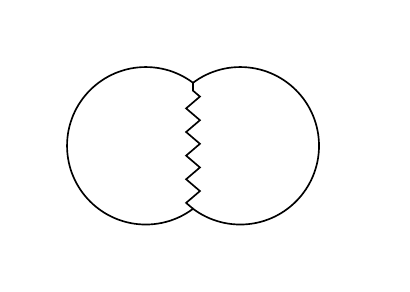
\begin{tikzpicture}
                        \begin{scope}
                            \clip (-1.5,-1.5) rectangle (0.6,1.5);
                            \draw [semithick] (0,0) circle(1cm) node [xshift=-0.2cm]{$\calL$};
                        \end{scope}
                        \draw [semithick,decorate, decoration={zigzag, segment length=3mm}] (0.6,-0.8) -- (0.6,0.8);
                        \begin{scope}
                            \clip (0.6,-1.5) rectangle (3,1.5);
                            \draw [semithick] (1.2,0) circle(1cm) node [xshift=0.2cm] {$\overline{\calL}$};
                        \end{scope}
                        % \draw [semithick,decorate, decoration={zigzag, segment length=3mm}] (0.7,-0.8) -- (0.7,0.8);
                    \end{tikzpicture}
                \end{center}
            }

            % \only<11->
            % {
            %     \begin{corollary}
            %         \alert{No subclass} of WSTS beyond REG is closed under complementation.
            %     \end{corollary}
            % }
        }
        \only<12->%
        {%
            \textbf{Proof:}

            Given $\lang{A_1}, \lang{A_2}$ disjoint WSTS languages.

            \begin{enumerate}
                \item<13-> Show that we can assume \wolog that $A_2$ is \alert{deterministic}.
                \item<14-> Find  \alert{safe inductive invariant} for $A_1 \times A_2$.
                \item<15-> Find a \alert{finite representation} of the invariant using \alert{ideals}.
                \item<16-> Convert this representation into an NFA defining a regular separator.
            \end{enumerate}
        }
    \end{overlayarea}
\end{frame}

\end{document}
